\Chapter{THE APPROACH AND STUDY DEFINITION}\label{sec:Theme1}

%TOTAL = 15 pages

\section{The Approach}

%2 pages

This section will describe the steps followed to design \ac{TEDIOUS}, our proposed machine learning detector to identify design technical debts to self-admit. It will also define its characteristics, how it works and how to use it. \ac{TEDIOUS} works at method-level since it is typically the granularity at which developers introduce \ac{SATD}, as proven by \citet{MaldonadoS15} and \citet{PotdarS14}. In other terms, it is able to define whether a method contains a design technical debt or not. Class-level granularity would be to coarse because technical debts normally admitted by developers are related to specific and punctual issues in the source code. Additionally, a class could contain a \ac{TD} but it would be impossible to precisely identify the source of the problem since a class contains several methods and \ac{LOC}. \par 

\begin{figure}[t]
	\centering
	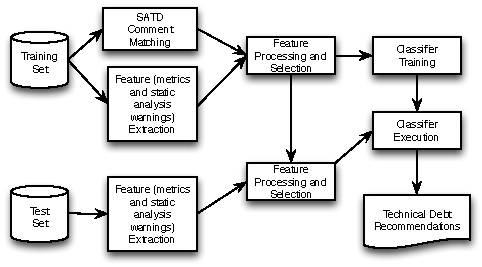
\includegraphics[width=\linewidth]{figs/approach.pdf}
	\caption{Proposed approach for recommending SATD.}
	\label{fig:approach}
	\vspace{-4mm}
\end{figure}

\ac{TEDIOUS} works as shown in Figure \ref{fig:approach}. Two datasets are required as inputs: the training set and the test set. The training set contains labeled data, which his source code from a project where technical debts are known and have been self-admitted through comments. The test set contains unlabeled data, which can be any source code under development or already released where \ac{TEDIOUS} can attempt to recommend where \ac{TD} should be self-admitted or where source code should be improved. \par 
	
For the training set, various kinds of metrics and static analysis warnings are extracted from the source code as well as \ac{SATD} methods in order to build an oracle to train the model. These labeled \ac{SATD} methods are essential for the machine learner since supervised learning is performed, meaning each method is labeled as true or false. It is true when the method is a \ac{TD} and false if it is not. \par 

Once all the information is extracted, feature preprocessing and selection is applied. Multi-collinearity, a phenomenon occurring when two predictor variables are highly correlated, meaning that one can be linearly predicted by the other, is dealt with. Feature selection is applied to retain only the most relevant variables to train the predictor. Finally, re-balancing is performed to address the issue of the low amount of positive examples, \textit{i.e.} \ac{SATD} methods. With the preprocessed features and the oracle now defined (each method is labeled as \ac{SATD} or not), the machine learners can be trained. \par 

In parallel, the test set is also being prepared. The same features are extracted from the source code but no \ac{SATD} matching is required since the data is unlabeled. \ac{SATD} are only required for the oracle, which is used for training the models. A similar feature filtering is applied, except for the re-balancing since it is only required on the labeled data. With both the test set and the previously trained classifier, predictions can be made on the test set in order to recommend when to self-admit technical debts. \par

Each step of the process will be described in the following sections. Firstly, the features used in more details: source code metrics and warnings raised by static analysis tools. Secondly, the method employed to identify \ac{SATD}. Thirdly, the feature preprocessing: multi-collinearity, feature selection and re-balancing. Finally, the training and application of the machine learning models.

\subsection{Features}

%3 pages

Three pieces of information extracted from the source code are necessary to accurately describe the source code: structural metrics, readability metrics and warnings raised by static analysis tools. There are reasons these specific characteristics were retained to describe the source code. The structural metrics are essential to capture symptoms of complex, heavily couples and poorly designed code. These metrics explain the quality of the implementation and the software's design. The readability metrics quantify symptoms of poorly documented code or hard to read and understand. Warnings from static analysis tools are related to more specific bad choices rather than globally bad code. They are issues which could lead to low maintainability and understandability of the code or which could potentially introduce defects in the future. In the following sections, these metrics and warnings are described more in depth.

\subsubsection{Source Code Metrics}

Source code metrics are extracted to characterize its size, coupling, complexity and number of comments for readability. Nine source code metrics are used. To define the size, metrics like \ac{LOC} or number of statements are calculated. For coupling, a metric such as number of call sites is computed. For complexity, McCabe cyclomatic complexity \citep{mccabe1990reverse}, number of defined variables, number of expressions and number of identifiers are calculated. It is important to know that not all comments are considered. \ac{SATD} related comments are ignored in the empirical evaluation to avoid \ac{TEDIOUS} becoming a self-prophecy. This issue will be covered later in the study design. \par

Firstly, to extract those source code metrics, an XML representation of the Java source code was generated using the srcML tool \citep{CollardKM03} and metrics' computation was applied to it. \textbf{SHOW IMAGE OF XML REPRESENTATION. SHOW IMAGE OF PSEUDOCODE AND EXPLAIN IT. VOIR PDF DU COURRIEL DANS DROPBOX.} It was also required to link comments to their related methods. The rule used was that any comments directly preceding or inside a method was assigned to it, rather it be a block of comments or just a single line. This step is essential to be able to classify which method is a \ac{SATD} and which one is not. Some methods were excluded from our analysis because they did not fit the context of our study, namely getter and setter methods since they are irrelevant with design debts. To do so, we looked for method prefixes matching \emph{get} or \emph{set} and made up from at least a single line of code. When these two criteria were covered, the method was removed from the dataset. \par 

Secondly, to extract the code readability metric, we use the one proposed by \citet{Buse:tse2010} and its related tool, based on a machine learning approach. This metric is based on specific characteristics of the source code: indentation, line length, identifier length, comment density, and the use of keywords and operators. The tool was also designed using feedback from human annotators, they were asked to rate the readability of code snippets, that was then used to classify snippets as "less" or "more" readable. A value between 0 and 1 is then computed based on these characteristics, 1 being the highest readability. The readability metric was considered relevant because, as mentioned by \citet{BavotaR16}, code readability is strongly correlated with the introduction of technical debts. Code that is difficult to read is consequently difficult to maintain and understand \citep{Buse:tse2010} thus more likely to contain \ac{TD}.

\subsubsection{Warnings Raised by Static Analysis Tools}

Warnings raised by static analysis tools are essential to detect poor coding practices, which are also related to the introduction of technical debts. We cannot directly relate a single flagged practice to a \ac{TD}. However, we can wonder if several flags are justifiable or not, and if they can be caused by the presence of a \ac{TD} in the source code. Having this hypothesis in mind, we used two popular static analysis tools, namely CheckStyle and PMD. Firstly, CheckStyle \citep{checkstyle} is widely used to check the adherence to coding standards and pieces of code that are potentially smells. It performs its analysis based on a configuration file, which can be modified at the discretion of the users. For our study, the default configuration containing code styles defined by Oracle and 43 checks was used. PMD \citep{pmd} main goal is to find common programming flaws such as unused objects, unnecessary catch blocks or incomprehensible naming. Similarly to CheckStyle, the default configuration was used, which contains 168 checks. Several reasons explains the choice of these two static analysis tools: they are adopted by \ac{OSS} \citep{BellerBMZ16}, they provide a wide range of warnings related to code styles and programming practices and they can be executed on source code statically. It is important to know that \ac{SATD} comments were removed when performing the analysis.

\subsection{Identification of Self-Admitted Technical Debt}

%0.5 page

As mentioned previously, the purpose of this study is not to propose a novel approach to detect \ac{SATD} using information from comments. Previous work has been completed aiming to address this issue by using pattern matching \citep{MaldonadoS15}, \citep{PotdarS14} or \ac{NLP} combined with machine learners \citep{maldonado17}. However, we still needed a dataset with methods tagged as design debt to train our machine learning models. \citet{maldonado17}, which worked on the \ac{NLP} approach, published a dataset of 10 open source projects annotated with methods tagged as technical debt or not. We used this dataset for our machine learning models and only the design debts were retained.

\subsection{Feature Preprocessing}

%3 pages

Several characteristics have been extracted from the source code, however, not all of them are relevant or necessary to train our models. Some clean up have to be done to reduce the size of the data input and improve the training phase. Multi-collinearity have to be dealt with, feature selection as to be applied as well as training set re-balancing. \textbf{SHOW IMAGE OF PSEUDOCODE AND EXPLAIN IT. FAIRE UN GRAPH STYLE LE PROCESS AU COMPLET. UN CARRE = UNE SOUS SECTION.}

\subsubsection{Multi-Collinearity}

We computed a lot features to characterize the source code of the projects, however, some of them can be strongly correlated and vary in the same way. Keeping these pairs of features would cause redundancy since they can be mutually linearly predicted. That is why, when facing a duo of such features, we only keep the one that better correlates with the dependent variable, the \ac{SATD} methods. The \emph{varclus} function in R, from the \emph{Hmisc} package, was used to help us achieve this preprocessing. This function performs a hierarchical cluster analysis of features to detect when two variable are positive based on similarity measures. It is mainly used to assess collinearity and redundancy, consequently resulting in data reduction. Hoeffding D statistic, squared Pearson or Spearman correlations measures can be applied. In this study, the Spearman's $\rho$ rank correlation measure was retained. To identify the problematic duos, the cluster tree has to be cut at a particular level of $\rho^2$, which represents the correlation value. In our case, a value of $\rho^2=0.64$ was used since it corresponds to a strong correlation \citep{Cohen-1988}.

\subsubsection{Feature Selection and Normalization}

Some features will vary a lot or not at all between methods. These features are not useful to build a predictor because they can't be used as proper learning variables, they won't be determinant compared to all the other features. The process of selecting only a relevant subset of all possible features is called feature selection. Several reasons can justify going through this selection: improving the prediction performance of machine learning models, improve the speed and cost-effectiveness of predictors, and simplify the models to better understand and interpret the underlying process behind the dataset generation \citep{guyon2003introduction}. \par 

The \emph{RemoveUseless} filter implemented in Weka \citep{hall2009weka} was used to perform feature selection. It looks for features that never vary or features that vary too much. For the latter, it looked for features that had a percentage of variance above a specific treshold, which was set to 99\%. \par 

In addition to feature selection, the metrics were also normalized. Several projects were analyzed, all having significant differences in complexity and size characteristics. Those aspects of the dataset will be covered in the study definition section. This normalization is necessary to reduce the effect of those differences on the predictor's training and to achieve good cross-project prediction performance.

\subsubsection{Re-Balancing}

To build performing predictors, a quality training set must be fed to the machine learner. One important aspect is to have a balanced dataset, which means having as much as possible an equal number of positive and negative examples, in our context, as many \ac{SATD} tagged methods as clean methods. This is a serious problem in our dataset since the vast majority of methods are not technical debts (this will be discussed more in depth in the next section), only a minority contain \ac{SATD}. There are two ways to address this issue: under-sample the majority class (methods with no \ac{SATD}) or over-sample the minority class (\ac{SATD} tagged methods). Since the training set is so highly unbalanced, the number of instances of the minority class is excessively small, the second option was favored. In fact, under-sampling would result in a very small training set. To apply over-sampling, artificial instances of \ac{SATD} methods must be generated from the existing ones. To do so, Weka provides a tool to perform over-sampling, called\ac{SMOTE} \citep{chawla2002smote}, which combines under-sampling the majority class and over-sampling the minority class to achieve improved classifier performance.

\subsection{Building and Applying Machine Learning Models}

%0.5 page
 We extracted various metrics, we identified \ac{SATD} methods and we performed a preprocessing on features, the only remaining step is building and applying the machine learning models. Two sets are required: the training set and testing set. The training set contains the methods with their corresponding features and an additional variable to tag them as positive or negative (\ac{SATD} or not). It is used to build the models. The testing set contains the same methods with the corresponding features, but not the variable tagging the methods because we want to test the prediction performance from a blank dataset. We experimented with five types of machine learners in Weka \citep{hall2009weka}: Decision Trees (J48), Bayesian classifiers, Random Forests, Random Trees, and Bagging with Decision Trees. Only the default configurations were used, however, further work could be made by trying to optimize these configurations.
 
 \textbf{SHOW IMAGE OF PSEUDOCODE AND EXPLAIN IT. VOIR LE ECLIPSE PROJECT QUE FIORELLA A ENVOYE.} Figure x.x provides an overview of the machine learning process.
	
\section{Study Definition}

0.5 page

\subsection{Dataset}

2 pages

\subsection{Analysis Method}

3.5 pages